\documentclass{article}

\usepackage[a4paper,top=2.5cm,bottom=2.3cm,left=2.0cm,right=1.5cm]{geometry}
\usepackage{tikz}
\usetikzlibrary{positioning,shapes,shadows,arrows,chains}
\usetikzlibrary{arrows,fit,backgrounds}
\usetikzlibrary{shadows.blur}

\begin{document}


\begin{tikzpicture}[remember picture,
      inner/.style={circle,draw=blue!50,fill=blue!20,thick,inner sep=3pt},
      outer/.style={draw=green,fill=green!20,thick,inner sep=10pt}
  ]
  \node[outer,draw=green] (A) {
    \begin{tikzpicture}
      \node [inner,draw=blue] (ai)  {A1};
      \node [inner,draw=blue,below=of ai] (aii) {A2};
      \node [inner,draw=blue,right=of aii] (aiii) {A3};
      \draw[red,thick] (ai) -- (aii) -- (aiii) -- (ai);
    \end{tikzpicture}
  };
  \node[outer,draw=green,right=of A] (B) {
    \begin{tikzpicture}
      \node [inner,draw=blue] (bi)  {B1};
      \node [inner,draw=blue,below=of bi] (bii) {B2};
      \node [inner,draw=blue,right=of bii] (biii) {B3};
      \node [inner,draw=blue,right=of bi] (biv) {B4};
      \draw[red,thick] (bi) -- (bii) -- (biii) -- (biv) -- (bi) -- (biii);
    \end{tikzpicture}
  };
  \draw[thick,orange,->] (ai) -- (bii);
  \draw[orange,->] (aiii) -- (bi);
  \draw[orange,->] (A.90) -- ($(A.90)+(0,1)$) -| (B);
\end{tikzpicture}


\newsavebox{\mybox}
\sbox{\mybox}{%
   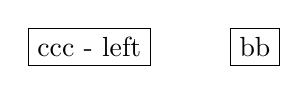
\begin{tikzpicture}[
                element/.style={draw=black, fill=white}
            ]
        \node(b)[element]{bb};
        \node(c)[element, left=of b]{ccc - left};
   \end{tikzpicture}
 }

\newbox\picbox
\def\groupnode(#1)[#2]#3{
    \sbox{\mybox}{%
        \begin{pgfinterruptpicture}
        \begin{pgfinterruptboundingbox}
            %Sub-\begin{pgfpicture}
            %\mbox{
                \begin{tikzpicture}[remember picture,element/.style={draw=black, fill=white}]
                    #3
                \end{tikzpicture}
            %}
            %\end{pgfpicture}
        \end{pgfinterruptboundingbox}
        \end{pgfinterruptpicture}
    }
    \pgfinterruptpicture% 
      % Interrupt the picture and put the graph in a box.
      \global\setbox\picbox=\hbox{\pgfpicture%
         % Set default tree options
         \tikzset{every node/.style={circle, draw, inner sep=0.0625cm}, 
           level distance=0.5cm, sibling distance=.5cm}%
          #3
        \endpgfpicture}%
      \endpgfinterruptpicture%
    \node(#1)[#2]{
        \usebox{\picbox}
    };
}



\begin{tikzpicture}[
        element/.style={draw=black, fill=white},
        group/.style={draw=black, rounded corners, fill=white},
        pics/grouped_contents/.style = {
            code = {
                #1
            }
        },
        pics/grouped/.style args={#1#2#3}{
            code = {
                \pgfinterruptpicture% 
  % Interrupt the picture and put the graph in a box.
  \global\setbox\picbox=\hbox{\pgfpicture%
     % Set default tree options
     \tikzset{every node/.style={circle, draw, inner sep=0.0625cm}, 
       level distance=0.5cm, sibling distance=.5cm}%
    %  
    \endpgfpicture}%
  \endpgfinterruptpicture%
  % Put box in a separate node otherwise some parameters
  % (e.g., dashing) will be inherited by the picture in the \picbox.
  \node(test) {test};
  \node [outer sep=0pt,below=of test] (@) {\copy\picbox}; 
  \begin{scope}[local bounding box=group_cnodegroup1]
  #3
  \end{scope}
  \node [draw, fit=(nodegroup1), inner sep=0pt, dashed] {};
  %\node [fit=(@)(title)] {};
            }
        }
    ]
    
    \node(main_a)[element]{MAIN A};
    \groupnode(group_a)[group, below=of main_a]{
        \node(b)[element]{bb};
        \node(c)[element, left=of b]{ccc - left};
    };
    \node(group_a_aux_r)[element,right=of group_a]{Aux Group Right};
    \node(group_a_aux_l)[element,left=of group_a]{Aux Group Left};
    \node(group_a_aux_b)[element,below=of group_a]{Aux Group Bottom};

    \draw[->,red] (main_a) -- (group_a);
    \draw[->,red] (group_a) -- (group_a_aux_r);
    \draw[->,red] (group_a) -- (group_a_aux_l);
    \draw[->,red] (group_a) -- (group_a_aux_b);
    
    \groupnode(group_b)[group, right=of group_a_aux_r]{
        \node(d)[element]{dddd};
        \node(e)[element, left=of d]{eeee - left};
    };
    
    %\pic [below=of group_b] {grouped={aaabcac}{asdas}{\node {XXXXX};}};
    \pic(group_c) [below=of group_b] {grouped={Group c}{asdas}{
        \node(b)[element]{bb};
        \node(c)[element, left=of b]{ccc - left};
        \node(a)[element, right=of b]{ccc - right};
        \draw[->,green] (c) -- (b);
    }};
    
    %code below fails - second image!!
    \node(aux_b)[element,right=of b,draw=blue]{Aux B};
    \node(aux_c)[element,left=of c,draw=blue]{Aux C};
    \draw[->,blue] (b) -- (aux_b);
    \draw[->,blue] (c) -- (aux_c);
    
    
    \draw[->,green] (c) -- (d);
    
    \draw[->,purple] (group_ca) -- (main_a);
\end{tikzpicture}

\begin{tikzpicture}[
        element/.style={draw=black, fill=white},
        group/.style={draw=black, rounded corners, fill=white},
        pics/grouped_contents/.style = {
            code = {
                #1
            }
        },
        pics/grouped/.style args={#1#2#3}{
            code = {
              \node(test) {test};
              \node [outer sep=0pt,below=of test] (@) {\copy\picbox}; 
              \begin{scope}[local bounding box=#2nodegroup1]
              #3
              \end{scope}
             %\node [draw, fit=(nodegroup1), inner sep=0pt, dashed] {};
              %\node [fit=(@)(title)] {};
            }
        }
    ]
    
    \node(main_a)[element]{MAIN A};

    %\pic [below=of group_b] {grouped={aaabcac}{asdas}{\node {XXXXX};}};
    \pic(group_c) [below=of main_a] {grouped={group_c}{asdas}{
        \node(b)[element]{bb};
        \node(c)[element, left=of b]{ccc - left};
        \node(a)[element, right=of b]{ccc - right};
        \draw[->,green] (c) -- (b);
    }};
    \pic(group_d) [right=of main_a] {grouped={group_d}{asdas}{
        \node(b)[element]{bb};
        \node(c)[element, left=of b]{ccc - left};
        \node(a)[element, right=of b]{ccc - right};
        \draw[->,green] (c) -- (b);
    }};
\end{tikzpicture}

\def\groupnoded(#1)[#2]#3{
  \begin{scope}[local bounding box=#1,#2]
          #3
  \end{scope}
  \node [draw, fit=(#1), inner sep=0pt, dashed] {};
}

\begin{tikzpicture}[
        remember picture,
        element/.style={draw=black, fill=white},
        group/.style={draw=black, rounded corners, fill=white}
        ]
    \node(main_a)[element]{MAIN A};
    
  \groupnoded(group_a)[local bounding box=group_a,below of = main_a]{%, below=3cm of main_a]
        \node(b)[element]{bb};
        \node(c)[element, left=of b]{ccc - left};
  }
  
  \groupnoded(group_b)[local bounding box=group_b,shift={($(group_a.east)+(group_a.east)$)},anchor=west]{%, below=3cm of main_a]
        \node(d)[element]{bbasdasd};
        \node(e)[element, left=of d]{ccc - left xx};
  }

\end{tikzpicture}
\end{document}